% !Mode\dots ``TeX:UTF-8''
% !TEX root = ../root.tex
\section{Determining the online observability of \BCNs}
\label{sec:deter}
In this paper, we propose two approaches to determine the online observability of \BCNs. The first way is by using supertree and the second way is by using directed graph. The construction process of supertree and directed graph simulates deduction process mentioned before. We check the super tree based on the definition of online observability of \BCNs\ depth first or breadth first. When we find enough leaf nodes, we can make sure the \BCN\ is online observable. But when we use the super tree to find all paths to determine the initial state of a \BCN, we need to check the existence of loops when we build the super tree. And many nodes in the tree are repeated, these nodes will take a lot of time overhead and space overhead for us to build and check the super tree for \BCNs. Therefore, we proposed the second way to determine the online observability of \BCNs\ by using directed graph. By this way we can avoid checking the existence of loop and avoid checking repeated nodes. There are also other advantages which help us select the input better in the process of determining the initial state of a \BCN by the second way. All of these advantages will reduce time and space overhead to determine the initial state of a \BCN. In conclusion if a \BCN\ seems to be online observable we would check it earlier by using supertree. But if a  \BCN\ does not seem to be online observable we prefer to check it earlier by using directed graph. If we just want to find a path to determine the initial state of a \BCN\ we would check it by using supertree. But if we want find all paths to determine the initial state of a \BCN\ and make some optimizations in the process of determine the initial state we prefer to check it by using directed graph.

\subsection{Algorithm implemented by supertree} As we mentioned before, we can use the deduction function to determine the initial state of \BCNs. According to the definition of online observability we will alternately observe the output and decide the input in the process of determining the initial state of a \BCN. When the  cardinal number of the states set comes into be $1$ we can determine the initial state, and we stop deducing the initial state of \BCNs. According to this process, we can define the supertree for \BCNs. For convenience, we use the states set inside the node to represent the node, and output in the edge to represent the edge.
\begin{definition}[Super Tree]
The root node of the super tree is $\Delta_N$, the leaf nodes of the super tree are the nodes with cardinal number $1$ ($|S_i|=1$). In addition to the leaf nodes, if a node $S_i$ in the $2k + 1$ ($k\in \mathbb{N}$) layer of the supertree and 
\[|\Ded\left(S_i,\varepsilon, o_j\right)|>0,\]
 then $\Ded\left(S_i,\varepsilon, o_j\right)$ is one of its son nodes, and $o_j$ is the edge from $S_i$ to $\Ded\left(S_i,\varepsilon, o_j\right)$ for each $o_j \in \Delta_Q$. If a node $S_i$ in the $2k+2$ layer of the supertree and  
\[|\Ded\left(S_i,i_p,\varepsilon\right)|=|S_i|,\] 
then $\Ded\left(S_i,i_p,\varepsilon\right)$ is the son node of $S_i$ and $i_p$ is the edge from $S_i$ to $\Ded\left(S_i,i_p,\varepsilon\right)$ for each $i_p \in \Delta_M$. 
\end{definition}

  \begin{figure}[thpb]
      \centering
      \framebox{\parbox{3in}{
		\centerline{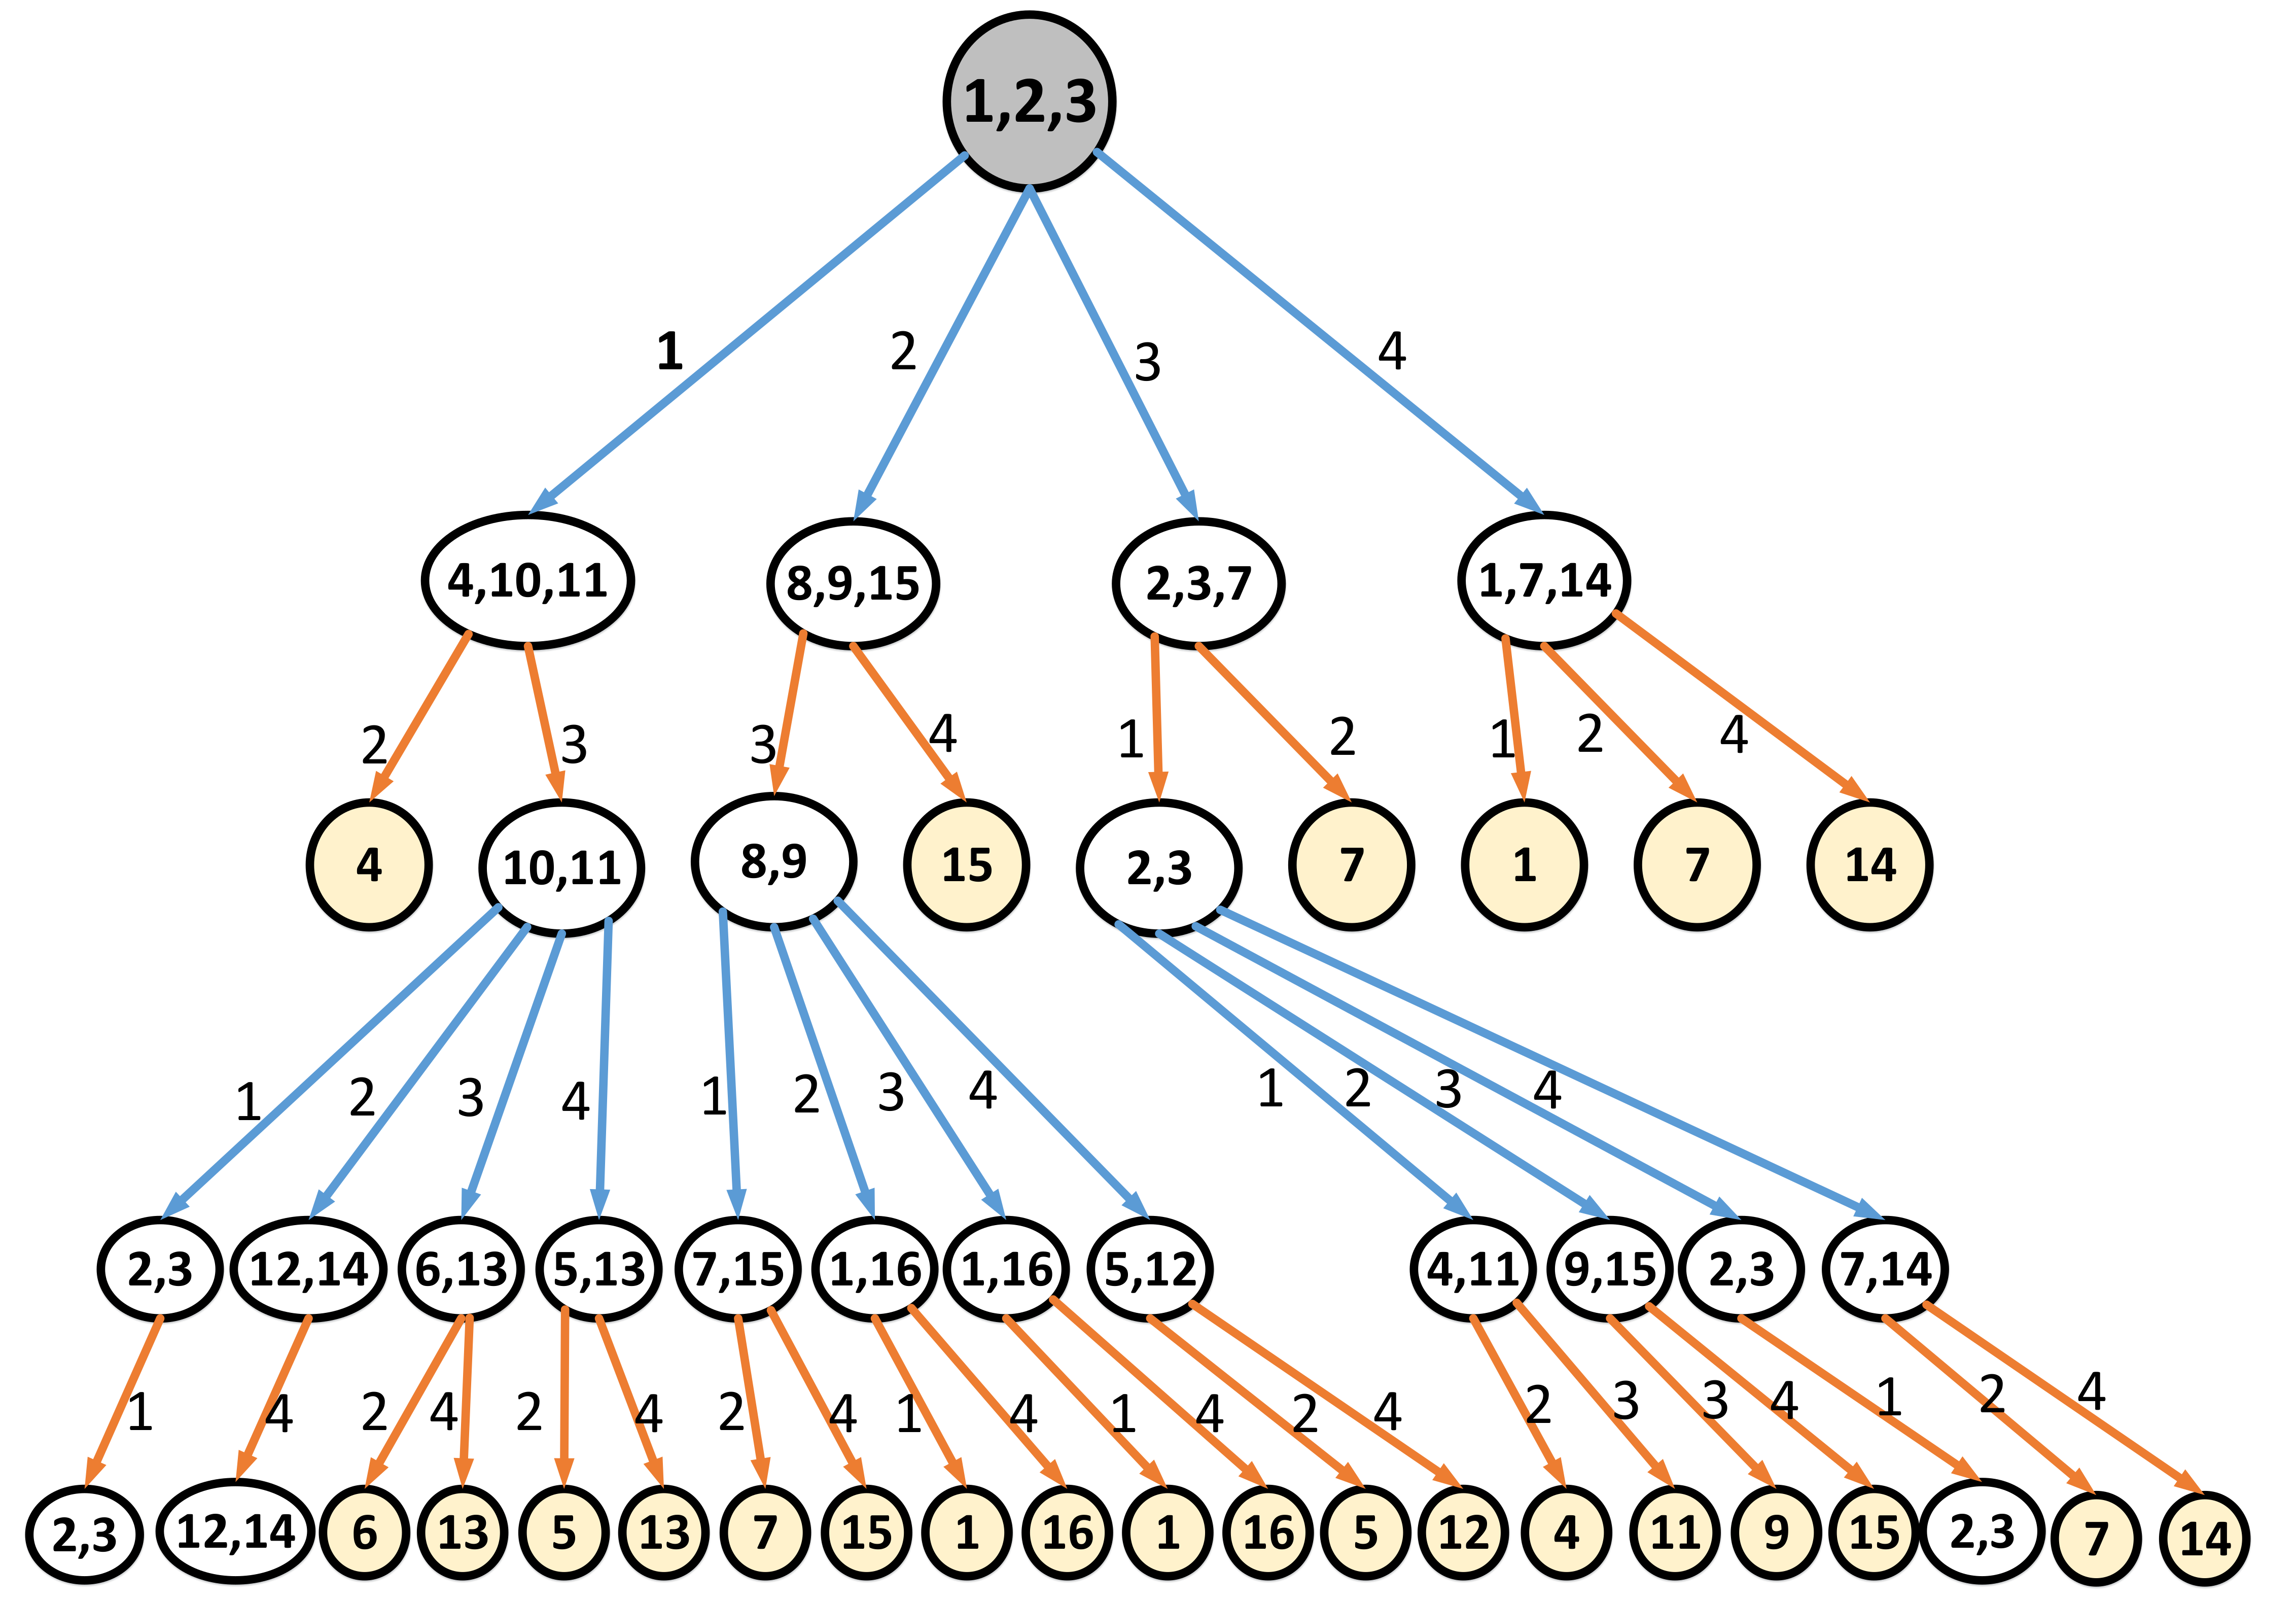
\includegraphics[scale=0.067]{figures/Fig3.png}}
	}}
      
      \caption{Branch of the super tree which represents $\{\delta_{16}^1,\delta_{16}^2,\delta_{16}^3\}$. The blue edges and orange edges show the observing output processes and deciding input processes, respectively. The yellow nodes are leaf nodes.}
      \label{fig:3}
   \end{figure}

At the beginning we infer that the possible states set is $\Delta_N$, thus the root node of the super tree is $\Delta_N$. When the cardinal number of the possible states set turns into $1$, we can determine the state of the \BCN. Therefore, the leaf nodes of the super tree are the nodes with cadinal number $1$. We observe the output of the \BCN\ to infer the possible states set of it at first. After that, we decide the input and infer the new possible states set of the \BCN. We alternately observe the output and decide the input untill we can determine the state of {\em BCN}. Therefore we use $\Ded\left(S_i,\varepsilon, o_j\right)$ to find son nodes for every $S_i$ in $2k+1$ layer, and using $\Ded\left(S_i,i_p,\varepsilon\right)$ to find son nodes for every $S_i$ in $2k+2$ layer. The formula $|\Ded\left(S_i,\varepsilon, o_j\right)|>0$ ensures the node $\Ded\left(S_i,\varepsilon, o_j\right)$ has meaning. The formula $|\Ded\left(S_i,i_p,\varepsilon\right)|=|S_i|$ guarantee we can determine the state of \BCN\ in the end ({\em Section \ref{sec:online}} {\em Equation \ref{equ:12}}).
\begin{example}
For example, the \BCN\ whose structure is depicted in Fig.\ref{fig:1}, and the updating rules of this \BCN\ is described as truth table in Fig.\ref{fig:2}. The Fig.\ref{fig:3} shows a branch of the super tree of this \BCN, and this branch has the root node $\{\delta_{16}^1,\delta_{16}^2,\delta_{16}^3\}$ (black node). The nodes represent the states sets, the blue edges represent the observing output processes, and the orange edges represent the deciding input processes. Only the yellow nodes are the leaf nodes, thus this branch is not completed. If we want to find all of the ways to determine the initial state of \BCN, we have to build all leaf nodes for the super tree of this \BCN. This process takes many additional time and space overhead. Especially when there are loops in the tree such as the $\{\delta_{16}^2,\delta_{16}^3\}$ in fourth layer and the $\{\delta_{16}^2,\delta_{16}^3\}$ in fifth layer that will form a loop. In this case we can never build the complete tree, thus we need to check the existence of loops and omit them. There are also some nodes take the same states set, then they will take some additional overhead as well. For instance there are two nodes take the same states set $\{\delta_{16}^1,\delta_{16}^{16}\}$ in the fifth layer. However, using super tree would be a lot easier than using directed graph if we only need to find a way to determine the initial state. For instance, when we find the leaf nodes $\delta_{16}^1$, $\delta_{16}^7$ and  $\delta_{16}^{14}$ in third layer by breadth-first algorithm, we can make sure that the states set $\{\delta_{16}^1,\delta_{16}^2,\delta_{16}^3\}$ is 1 step deterministic. Therefore, we could use this conclusion to determine the initial state of this \BCN. 
\end{example}   
\subsection{Algorithm implemented by directed graph}
To improve the shortcomings of the algorithm by using supertree, we proposed the algorithm by derected graph wich may takes less time and space overhead to determine the online observability of \BCNs. The most difference between supertree and derected graph is that supertree is built from the root node to leaf nodes. However, the derected graph is built from smaller nodes (contain fewer states) to larger nodes (contain more states). In addition, there is not any repeated node in the derected graph because any node only appears once in the directed graph. And even there are some loops in the derected graph, the loops can not prevent us from building the directed graph completely.

The construction algorithm of derected graph is shown in the {\em Algorithm.\ref{alg:1}}. The algorithm to build nodes used in the {\em Algorithm.\ref{alg:1}} is shown in the {\em Algorithm.\ref{alg:2}}.

\begin{algorithm}[h]
\caption{Algorithm to construct the directed graph of \BCNs}
\begin{algorithmic}[1]
\REQUIRE 
The algebraic forms of \BCN
\ENSURE  
The directed graph of \BCN
\STATE  $k=1$ (The number of states in the nodes)\
\STATE  $Ob=$ false (The online observability of \BCN)\
\STATE  $N_i$ (Node)\
\STATE  $i_p$ (Input)\
\STATE  $NodesArray$ (Nodes array)\
\STATE  $Sis$ (The suitable inputs set of $N_i$)\
\STATE {\sf buildnode}(k)
\STATE $k= k+1$
\WHILE {NodesArray={\sf buildnode}(k)!=Null}
\STATE NodesArray={\sf buildnode}(k)
\FOR{each $N_i\in NodesArray$}
\IF{$k==2$}
\STATE $Sis$ = $\Delta_M$ 
\ELSE

\STATE Find $Sis$ by other nodes

\ENDIF
\FOR{each $i_p \in Sis$}
\STATE Check $N_i$ by $i_p$
\STATE Build edges for $N_i$ 
\ENDFOR
\IF {$N_i$ has not any edge.}
\STATE $Ob=0$ 
\STATE return Null
\ENDIF
\ENDFOR

\STATE $k= k+1$
\ENDWHILE
\STATE $Ob=1$ 
%\STATE return $Ob$
\STATE return $NodesArray$
\end{algorithmic}
 \label{alg:1}
\end{algorithm}
 %The algorithm to build nodes used in the Algorithm.\ref{alg:1} is shown in the Algorithm.\ref{alg:2}.
\begin{algorithm}[h!]
\caption{{\sf buildnode}(int k)}
\begin{algorithmic}[1]
\REQUIRE 
The number of states in the nodes $k$
\ENSURE  
The nodes with $k$ states whose corresponding outputs are the same%, and the outputs of $p$ states inside one node are the same.
%\STATE {\sf buildnode}(int p)
%\STATE  \{ 
%\dfSTATE $p=p+1$\
\STATE  Build all nodes with $p$ states %(whose outputs are the same)\

\IF{Failed to build} 
\STATE  return Null
\ELSE 
\STATE  Classify these nodes
\STATE Sort the states in these nodes
\STATE Sort these nodes%(For example, the nodes $\{\delta_{16}^1,\delta_{16}^2\}$, $\{\delta_{16}^1,\delta_{16}^3\}$ and $\{\delta_{16}^2,\delta_{16}^3\}$ shown in {\em Fig.\ref{fig:4}}. )
\STATE return nodes
\ENDIF 
%\STATE \}
\end{algorithmic}
 \label{alg:2}
\end{algorithm}

Some details in {\em Algorithm.\ref{alg:1}} and {\em Algorithm.\ref{alg:2}} are as follows:
\begin{itemize}
\item Build all nodes with $k$ states: Firstly, we classify all states by their corresponding outputs, then we have all of states sets. The states set contains all states have the same corresponding outputs. Secondly, we compare $k$ with the cardinal number $Car$ of each states set $S_i$ we built before. If $k$ greater than $Car$, then we could not get $k$ states from this states set $S_i$. Else we can get $C_{Car}^k$ sets with $k$ states from this states set. Finally, we use all of states sets to build nodes we need. 
 \item Sort the states in these nodes and sort these nodes: For example, the nodes $\{\delta_{16}^1,\delta_{16}^2\}$, $\{\delta_{16}^1,\delta_{16}^3\}$ and $\{\delta_{16}^2,\delta_{16}^3\}$ shown in Fig.\ref{fig:4}. 
  \item Find $Sis$ by other nodes: The node $N_i$ with $k$ sorted states inside it, then we can use the first $k-1$ states, the last $k-1$ states and the first and last two states to find the nodes we need. And then use these three nodes to find $Sis$ for $N_i$. For example, we can search right inputs sets which make $\{\delta_{16}^4,\delta_{16}^5,\delta_{16}^6\}$, $\{\delta_{16}^5,\delta_{16}^6,\delta_{16}^7\}$ and $\{\delta_{16}^4,\delta_{16}^7\}$ $k$-step deterministic at first. After that, take the intersection of these sets to be the suitable inputs set of $\{\delta_{16}^4,\delta_{16}^5,\delta_{16}^6,\delta_{16}^7\}$. 
  \item Check $N_i$ (with states set $S_i$ in it) by $i_p$: According to the order determined in previous steps, we check every node in order. If for one input $i_p$ (which belongs to suitable inputs set $Sis$) implies $|\Ded\left(S_i,i_p,\varepsilon\right)|<|S_i|$, we can make sure the $i_p$ is a wrong input. Else if for each $O_j \in \Delta_Q$, $|\Ded\left(S_i,i_p,o_j\right)|>0$ and $\Ded\left(S_i,i_p,o_j\right)$ is $k$-step deterministic then $I_j$ is a right input. Therefore, we can connect the node $S_i$ to each node $\Ded\left(S_i,i_p,o_j\right)$ with directed edge. The colour of directed edges represent its corresponding input. Else if there exist $o_j \in \Delta_Q$ and we can not make sure whether $\Ded\left(S_i,i_p,o_j\right)$ is $k$-step deterministic, we check it in the next round. 
\end{itemize} 

According the construction process, we have the definition of directed graph.
\begin{definition}[Directed Graph]
Every node $S_i$ in the directed graph is $k$-step deterministic, and there are no duplicate nodes in the graph. For every distinct two $s_a, s_b \in S_i$ we have $Hs_a=Hs_b$. If $|S_i|=1$, then there are not edge from it to other nodes, else if there are exist one edge $i_p$ from it to one nodes then there exist $z$ ($z\ge 1)$ edges contain $i_p$ from it to nodes $S_1,\ldots,S_z$ that \[|S_i|= |S_1|+,\ldots,|S_z|\] and \[\Ded\left(S_i,i_p,\varepsilon\right)=S_1\vee,\ldots,\vee S_z.\]
\end{definition}

When we trying to build the directed graph for a \BCN, we check whether the nodes with fewer states are $k$-step deterministic first and then check whether the nodes with more states are $k$-step deterministic.  As the the nodes with fewer states are not $k$-step deterministic, the nodes with more states would not be $k$-step deterministic. Therefore, once we can find a node is not $k$-step deterministic we can know that $\Delta_N$ is not $k$-step deterministic and this \BCN\ is not online observable. Moreover, we can use the nodes with fewer states that are $k$-step deterministic to help us check the nodes with more states. For instance, if the node $S$ has two edges from it to two nodes $S_1$ and $S_2$, and we have $S_1$ and $S_2$ are $k$-step deterministic. In this case, we can make sure that the node $S$ is $k$-step deterministic.

Based on the definitions of existing four kinds of observability, we can also use the directed graph to determine the existing second and fourth kinds of observability. When we try to build bottom layer and penultimate layer of the directed graph, and there are exist some nodes in penultimate layer has no edges from it to other nodes. In this case this \BCN\ is not satisfied existing second observability. When we try to build edges for every layer, and if there exist one node whose right inputs set is not $\Delta_M$, then this BCN is not satisfied existing fourth observability.
\begin{figure}[thpb]
      \centering
      \framebox{\parbox{3in}{
		\centerline{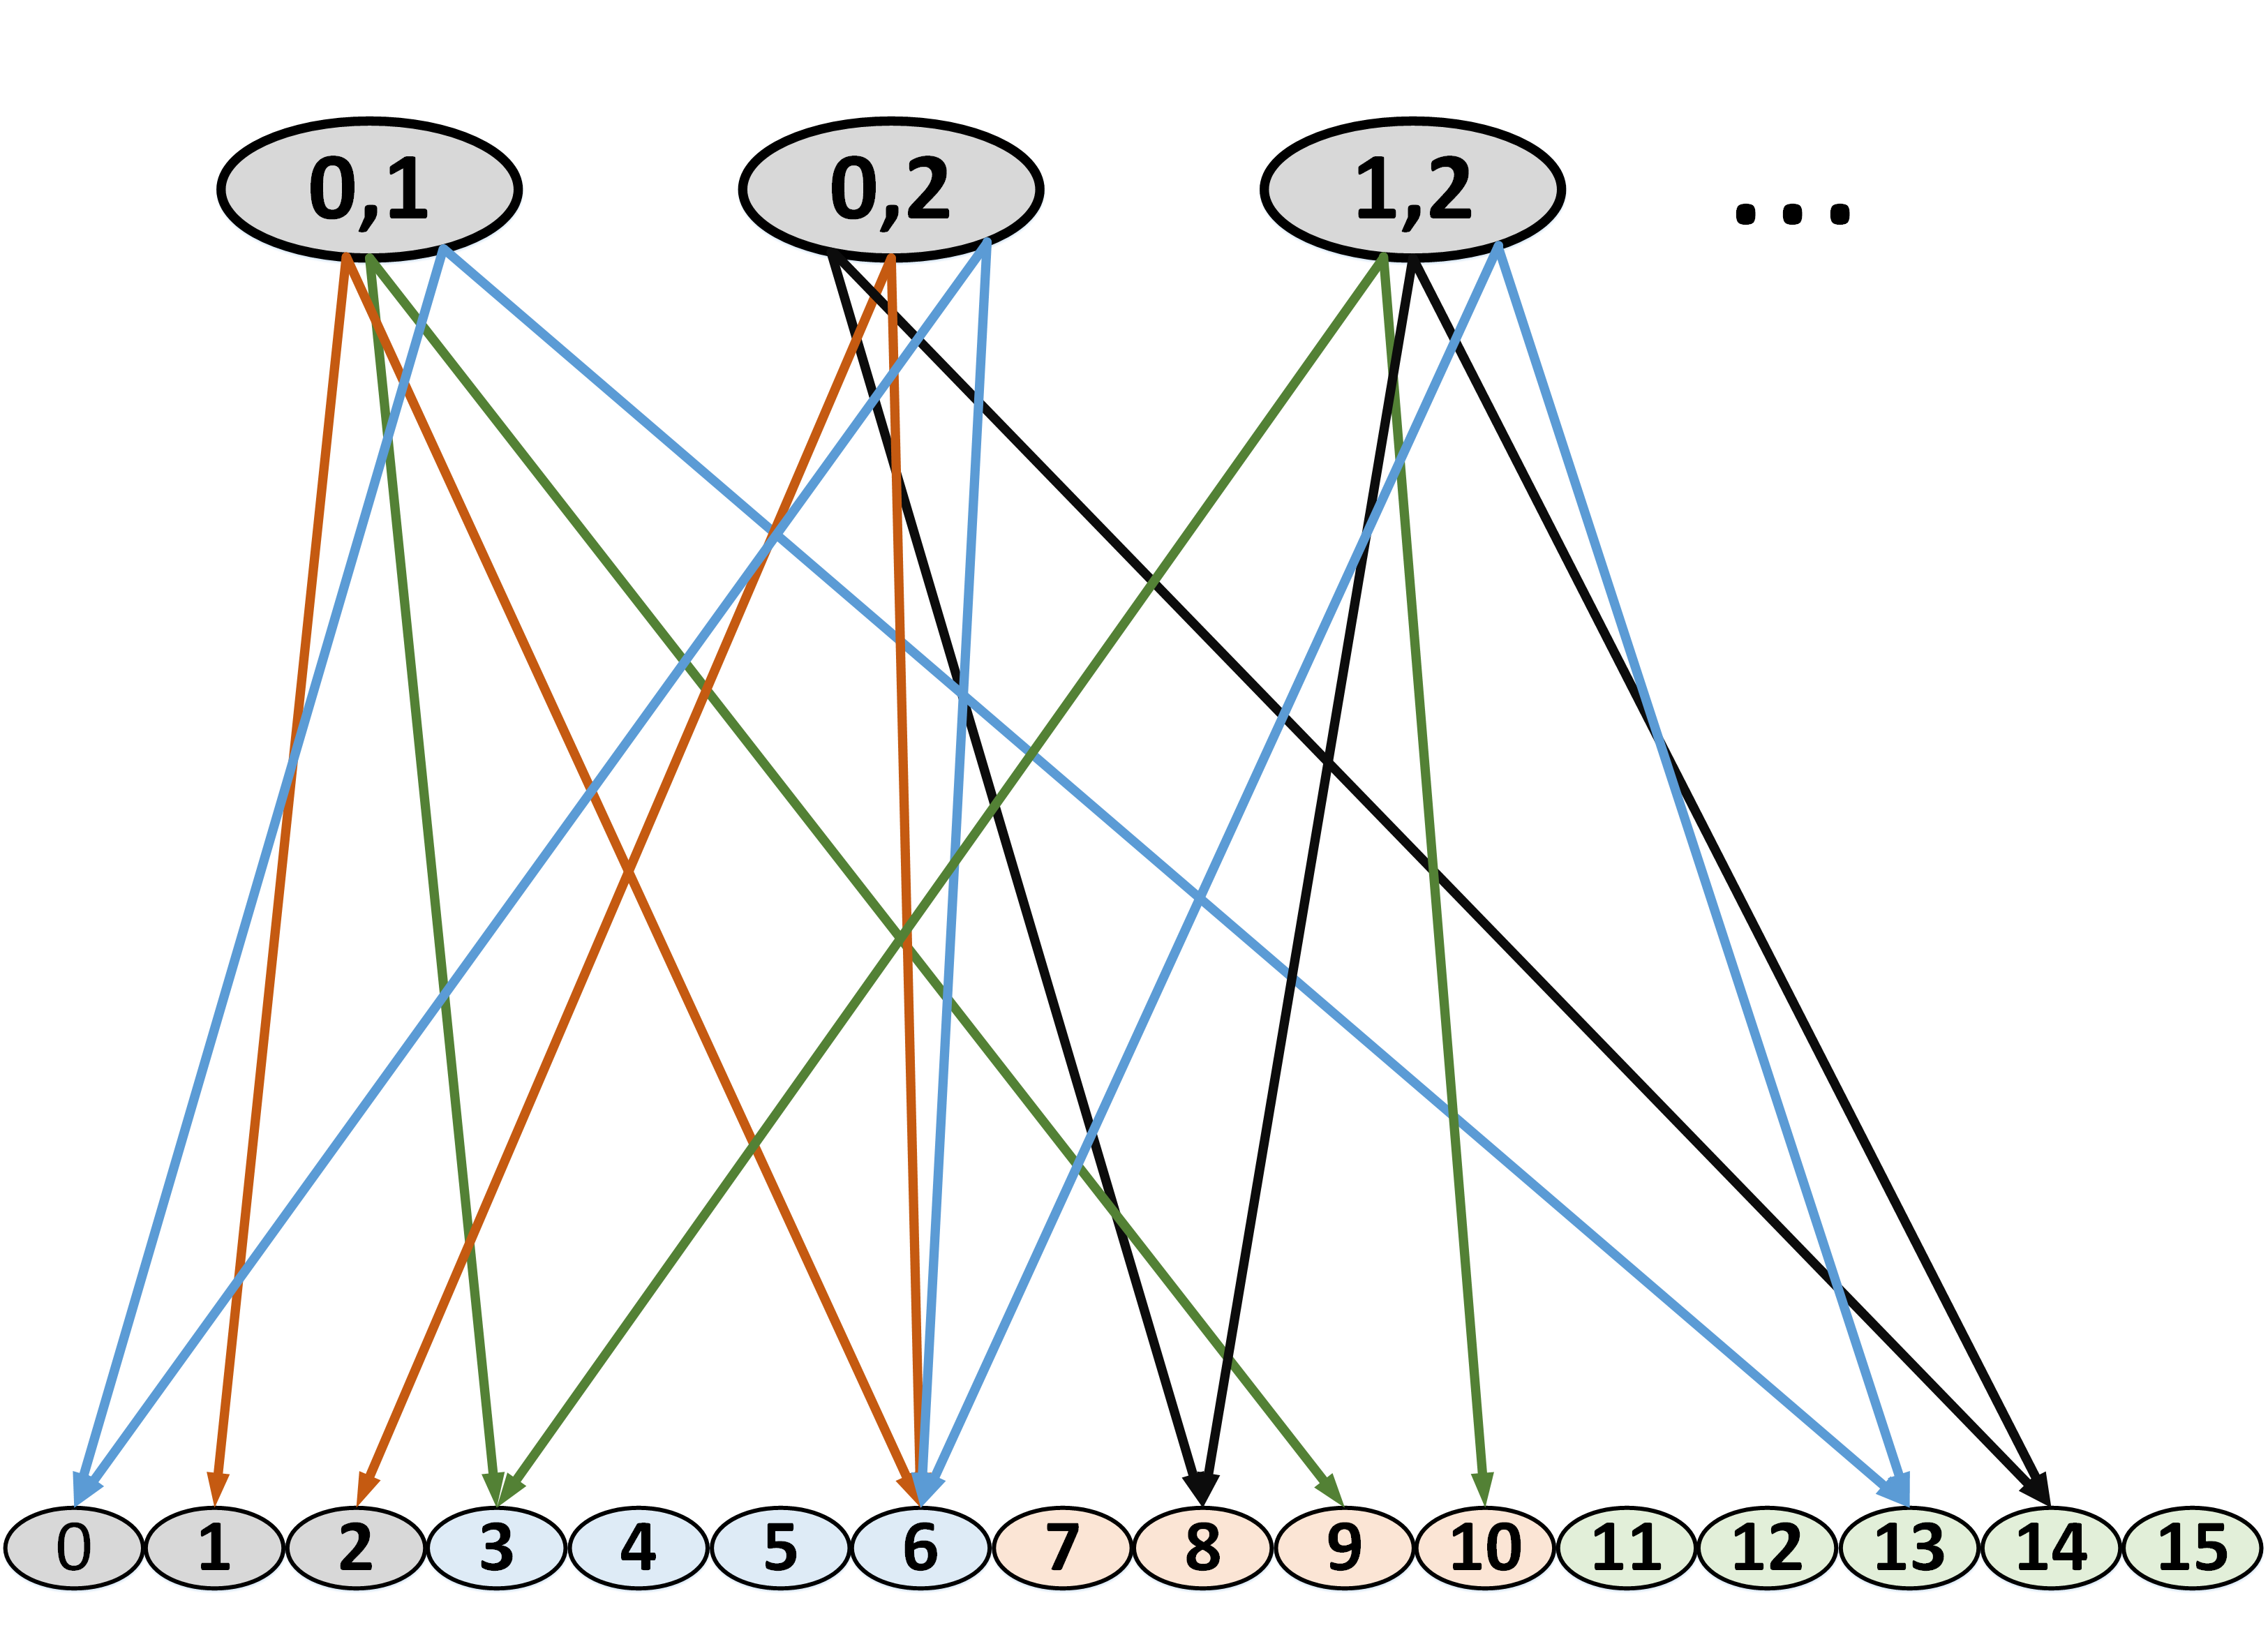
\includegraphics[scale=0.090]{figures/Fig4.png}}
	}}
      
      \caption{Part of the directed graph which represents $\{\delta_{16}^1,\delta_{16}^2\}$, $\{\delta_{16}^1,\delta_{16}^3\}$ and $\{\delta_{16}^2,\delta_{16}^3\}$. The green, black, orange, blue edges show the inputs $\delta_4^1$, $\delta_4^2$, $\delta_4^3$ and $\delta_4^4$ respectively.}
      \label{fig:4}
   \end{figure}
\subsection{Complexity analysis}
The algorithm by the directed graph is better than by supertree when we want to find all paths to determine the initial state of \BCNs. Therefore we analyze the complexity of this algorithm in this paper. We classify the states with their corresponding output. After that form the set of states set $\{S_1, S_2,\ldots,S_M\}$,  then every element in a states set has the same corresponding output. For each 
\[S_i\in\{S_1, S_2,\ldots,S_M\}\]
 then we have $Hs_k=\delta_{M}^i$ for every $s_k\in S_i$.

Firstly, we need to calculate the upper bound of the number of the states in the directed graph nodes $k$ we have.
\begin{equation}
\begin{split}
k_{upb}= \max(|S_1|,|S_2|,\ldots,|S_M|)
\end{split}
\end{equation}
The $k_{upb}$ is the maximum value of $|S_1|,|S_2|,\ldots,|S_M|$, because the states in the directed graph nodes should have the same corresponding output. Therefore, the $k_{upb}$ indicates the number of times we need to run the {\sf buildnode}(k) function.

Secondly, we need to calculate the number of nodes which with $k$ states:
\begin{equation}
\begin{split}
k_{non}= C_{|S_i|}^k+\ldots +C_{|S_p|}^k
\end{split}
\end{equation}
where $S_i\ldots,S_p\in\{S_1, S_2,\ldots,S_M\}$ and $|S_i|,\ldots,|S_p|\ge k$. The $k_{non}$ indicates the number of nodes which built by the {\sf buildnode}(k) function.

Thirdly we need to calculate the cardinal number of suitable inputs set of each node. Finally we need to calculate the time used to check whether a input which in the suitable inputs set of a node is a right input for this node.

After completing the previous steps, we calculate the complexity by layer by layer. The cardinal number of suitable inputs set of a node depends on the cardinal number of this node and the other three nodes used to find the suitable inputs set for it. And the time used to check whether an input is a right input for a node also depends on the updating rules of {\em BCNs}.

What is more, instead of taking $\Delta_M$ as the suitable inputs set for every node in thedirected graph, we use the other three nodes like $\{\delta_{16}^4,\delta_{16}^5,\delta_{16}^6\}$, $\{\delta_{16}^5,\delta_{16}^6,\delta_{16}^7\}$ and $\{\delta_{16}^4,\delta_{16}^7\}$ that are $k$-step deterministic to find the suitable inputs set for a node $\{\delta_{16}^4,\delta_{16}^5,\delta_{16}^6,\delta_{16}^7\}$ which with more than $2$ states. By this way we can  reduce the cardinal number of the suitable inputs set for every nodes with more than 2 states, and then reduce the time cost. 

The reason why we can use this method is that only the input which make the subset of $\{\delta_{16}^4,\delta_{16}^5,\delta_{16}^6,\delta_{16}^7\}$ $k$-step deterministic will make the $\{\delta_{16}^4,\delta_{16}^5,\delta_{16}^6,\delta_{16}^7\}$ $k$-step deterministic. Furthermore, using these three nodes will be a good way to cover all the 2-state subsets (which with cardinal number $2$) of $\{\delta_{16}^4,\delta_{16}^5,\delta_{16}^6,\delta_{16}^7\}$. For every subset $s_i$ with cardinal number $2$ included in $\{\delta_{16}^4,\delta_{16}^5,\delta_{16}^6,\delta_{16}^7\}$ will included in $\{\delta_{16}^4,\delta_{16}^5,\delta_{16}^6\}$, $\{\delta_{16}^5,\delta_{16}^6,\delta_{16}^7\}$ or $\{\delta_{16}^4,\delta_{16}^7\}$. This conclusion can help us to select the nodes we need when we seek the suitable inputs set for a node. But it is hard to analyze the complexity of this method, and it makes the complexity analysis of the algorithm by directed graph harder.

Therefore, it is hard to give a accurate complexity of the algorithm without the complete imformation of \BCNs. We just give a short introduction of complexity analysis in this paper, we may finish this work in the furture.
%Because the states in a nodes will have the same corresponding output, so we have the upper bound of the number of the states in a directed graph nodes $k$: We classify the states with their corresponding output and form the set of states with the same corresponding output, the greatest cardinal number of these set would be the upper bound of $k$. 